% id: 0353
% book: 쎈 중3-2 수학 · 03 원과 직선
% section: 유형 13 삼각형의 내접원
% figure: tikz:fig-0353
% answer: ③
% answer_source: 답지
% variant_level: 0 (원본 전사)
% 이 파일은 build.mjs 가 items.json 에서 만든다. 고칠 때는 items.json 을 고친다.
\smash{\raisebox{1.5mm}{\dmkichul{쎈 중3-2 수학 0353번 · 66쪽 · 대표문제}}}
\noindent\begin{minipage}[t]{0.58\linewidth}\vspace{0pt}\raggedright 오른쪽 그림에서 원~$\pt{O}$는 $\triangle\pt{ABC}$의 내접원이고 세 점~$\pt{D}$, $\pt{E}$, $\pt{F}$는 접점이다. $\seg{AB}=12\,\mathrm{cm}$, $\seg{BC}=14\,\mathrm{cm}$, $\seg{AC}=10\,\mathrm{cm}$일 때, $\seg{AD}$의 길이는?\end{minipage}\hfill\begin{minipage}[t]{0.4\linewidth}\vspace{0pt}\centering \resizebox{\ifdim\width>\linewidth\linewidth\else\width\fi}{!}{% 0353(본책 66쪽) — △ABC 의 내접원 O(접점 D, E, F), AB=12 cm, BC=14 cm, AC=10 cm. 답(AD)은 적지 않는다. 스캔 삽화를 TikZ 로 다시 그림.
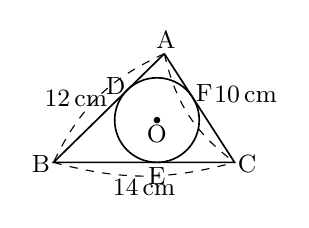
\begin{tikzpicture}[line width=0.6pt]
  \draw (1.408,1.380) -- (0.000,0.000) -- (2.300,0.000) -- (1.408,1.380);
  \draw (1.314,0.537) circle (0.537);
  \fill (1.314,0.537) circle (1.2pt);
  \draw[dashed, line width=0.4pt] (1.408,1.380) to[bend right=20] (0.000,0.000);
  \node[font=\small, inner sep=1.5pt] at (0.284,0.810) {$12\,\mathrm{cm}$};
  \draw[dashed, line width=0.4pt] (0.000,0.000) to[bend right=15] (2.300,0.000);
  \node[font=\small, inner sep=1.5pt] at (1.150,-0.320) {$14\,\mathrm{cm}$};
  \draw[dashed, line width=0.4pt] (1.408,1.380) to[bend right=20] (2.300,0.000);
  \node[font=\small, inner sep=1.5pt] at (2.440,0.860) {$10\,\mathrm{cm}$};
  \node[font=\small, inner sep=1.5pt] at (1.428,1.550) {A};
  \node[font=\small, inner sep=1.5pt] at (-0.160,-0.020) {B};
  \node[font=\small, inner sep=1.5pt] at (2.460,-0.020) {C};
  \node[font=\small, inner sep=1.5pt] at (0.789,0.970) {D};
  \node[font=\small, inner sep=1.5pt] at (1.314,-0.170) {E};
  \node[font=\small, inner sep=1.5pt] at (1.915,0.878) {F};
  \node[font=\small, inner sep=1.5pt] at (1.314,0.357) {O};
\end{tikzpicture}
}\end{minipage}\par
\begin{choices32}{$3\,\mathrm{cm}$}{$3.5\,\mathrm{cm}$}{$4\,\mathrm{cm}$}{$4.5\,\mathrm{cm}$}{$5\,\mathrm{cm}$}\end{choices32}
